\documentclass[prodmode,acmtoms]{acmsmall}
%  

% Package to generate and customize Algorithm as per ACM style
\usepackage[ruled]{algorithm2e}
\renewcommand{\algorithmcfname}{ALGORITHM}
\SetAlFnt{\small}
\SetAlCapFnt{\small}
\SetAlCapNameFnt{\small}
\SetAlCapHSkip{0pt}
\IncMargin{-\parindent}

% Metadata Information
\acmVolume{0}
\acmNumber{0}
\acmArticle{00}
\acmYear{0000}
\acmMonth{0}

%
%%% User-requested packages placed after this line %%%%%%%%%%%%%%%%%%%%%%%%%%%%
\usepackage{amsfonts,amssymb,amsmath}
\usepackage{booktabs,dcolumn}
\usepackage[T1]{fontenc}
\usepackage{mathtools}
\usepackage{enumerate,graphicx}
\usepackage{subfig}
\usepackage{multirow}
% \usepackage[center]{subfigure}
\numberwithin{equation}{section}
\usepackage{braket}                             %Provides \Set for typing sets
\usepackage{float}
\usepackage{subfig}


%%% User's macros placed after this line %%%%%%%%%%%%%%%%%%%%%%%%%%%%%%%%%%%%%%
%\IfFileExists{dsfont.sty}%
%\usepackage{dsfont}
\newcommand{\R}{\mathbb{R}}
\newcommand{\N}{\mathbb{N}}
\renewcommand{\phi}{\varphi}
\renewcommand{\epsilon}{\varepsilon}

\newcommand{\todo}[1]{\textbf{\textsc{\textcolor{black}{TODO: #1}}}}

%
\begin{document}
\markboth{C. Goll, T. Wick, and W. Wollner}{DOpElib: A Goal Oriented Software Library}

\title{DOpElib: A Goal Oriented Software Library for Computing PDEs and Optimization Problems}

\author{CHRISTIAN GOLL
\affil{University of Heidelberg}
THOMAS WICK
\affil{University of Heidelberg}
WINNIFRIED WOLLNER
\affil{University of Hamburg}}

%%%%%%%%%%%%%%%%%%%%%%%%%%%%%%%%%%%%%%%%%%%

\begin{abstract}
In this article, we describe the software library 
\textit{Deal.II Optimization Environment} (DOpElib).
The main feature of DOpElib is that it provides a unified interface to high level algorithms 
such as time stepping methods, nonlinear solvers and optimization routines. This structure ensures 
that first of all the user is required to write those sections of code that are specific to 
the considered problem. Second, the exchange of parts of the used routines is possible 
with the need for just a few lines of code to change.
The article illustrates performance and features 
of the software package by four numerical tests. 
\end{abstract}

%\category{C.2.2}{Computer-Communication Networks}{Network Protocols}

%\terms{Design, Algorithms, Performance}

%\keywords{Wireless sensor networks, media access control,
%multi-channel, radio interference, time synchronization}

%\acmformat{Zhou, G., Wu, Y., Yan, T., He, T., Huang, C., Stankovic,
%J. A., and Abdelzaher, T. F.  2010. A multifrequency MAC specially
%designed for  wireless sensor network applications.}

\begin{bottomstuff}
Author's adresses: C. Goll {and} T. Wick, Institut f\"ur Angewandte Mathematik, Universit\"at Heidelberg;
W. Wollner, Fachbereich Mathematik, Universit\"at Hamburg.
\end{bottomstuff}
                      

\maketitle
%%%%%%%%%%%%%%%%%%%%%%%%%%%%%%%%%%%%%%%%%%%


%%%%%%%%%%%%%%%%%%%%%%%%%%%%%%%%%%%%%%%%%%%
\section{Introduction}
\label{introduction}

\todo{Wie sehr wollen wir deal.II im ersten Satz hervorheben?}
\todo{Vorschlag von TW: 
The aim of the \textit{Deal Optimization Environment} (DOpElib) 
is to provide a software toolkit to solve forward PDE
problems as well as optimal control problems constrained by PDE. The
solution of a broad variety of PDE is possible in other software
libraries (like in deal.II, dune, or commercial solvers Ansys) 
as well, but
DOpE concentrates on a unified approach for both linear and nonlinear
problems by interpreting every PDE problem as nonlinear and applying a
Newton method to solve it. While deal.II leaves much of the work and many
decisions to the user, DOpE intends to be user-optimized by delivering
prefabricated tools which require from the user only adjustments connected
to his specific problem. The solution of optimal control problems with PDE
constraints is an innovation in the DOpE framework.
The focus is on the numerical solution of both stationary and nonstationary
problems which come from different application fields, like elasticity and
plasticity, fluid dynamics, and fluid-structure interactions.
}

The DOpElib project is 
based on the \textit{deal.II} \cite{deal} finite element library which has been developed
 initially by W. Bangerth, R. Hartmann, and G. Kanschat \cite{deal}.
Its main feature is to give a unified interface to high level algorithms such as 
time stepping methods, nonlinear solvers and optimization routines. 
We aim that the user should only need to write those parts
of the code that are problem dependent while all invariant parts of the algorithms
should be reusable without any need for further coding.
In particular, the user should be able to switch between various different 
algorithms without the need to rewrite the problem dependent code, though he or she will
have to replace the algorithm object with an other one. 

The authors acknowledge their past experience as well as discussions with 
the authors of the libraries 
Gascoigne/RoDoBo project, which was initiated by 
Roland Becker, Dominik Meidner,  and Boris Vexler \cite{rodobo}. 
From which some of the ideas to modularize the algorithms have arisen.

%%%%%%%%%%%%%%%%%%%%%%%%%%%%%%%%%%%%%%%%%%%%%%%%%%%
%The aim of DOpE is to provide a software toolkit to solve forward PDE
%problems as well as optimal control problems constrained by PDE. The
%solution of a broad variety of PDE is possible in deal.II as well, but
%DOpE concentrates on a unified approach for both linear and nonlinear
%problems by interpreting every PDE problem as nonlinear and applying a
%Newton method to solve it. While deal.II leaves much of the work and many
%decisions to the user, DOpE intends to be user-optimized by delivering
%prefabricated tools which require from the user only adjustments connected
%to his specific problem. The solution of optimal control problems with PDE
%constraints is an innovation in the DOpE framework.
%The focus is on the numerical solution of both stationary and nonstationary
%problems which come from different application fields, like elasticity and
%plasticity, fluid dynamics, and fluid-structure interactions.
%

At the present stage the following key features are supported by the library
\begin{itemize}
\item Solution of stationary and nonstationary PDEs in 1d, 2d, and 3d.
\item Various time stepping schemes (based on finite differences), 
  such as forward Euler, backward Euler,
  Crank-Nicolson, shifted Crank-Nicolson, and Fractional-Step-$\Theta$ scheme.
\item All finite elements of from deal.II including hp-support.
\item Several examples showing the solution of several PDEs including
   Poisson, Navier-Stokes, Plasticity and fluid-structure interaction problems. 
\item Self written line search and trust region newton algorithms for the 
   solution of optimization problems with PDEs \cite{NoWr00}
\item Interface to SNOPT for the solution of optimization problems with PDEs and
  additional other constraints.
\item Several examples showing how to solve various kinds of optimization problems
  involving stationary PDE constraints.
\item Mesh adaptation.
\item Different spatial triangulations for control and state variables.
\end{itemize}

The article is organized as follows. In Section
\ref{detailed_description} 
 
%The rest of this document is structured as follows: We start with an introduction in
%Chapter~\ref{chap:intro} where you will learn what is needed to run {\tt DOpElib}. 
%Further you will learn what problems we can solve and how all the different classes 
%work together for this purpose. This should help you figure out what the different classes
%do if you are in need of writing your own algorithm.
%
%Then assuming that you can work to your satisfaction with the algorithms already implemented
%we will show you how to create your own running example in Chapter~\ref{chap:howtoex}.
%This will be followed by a detailed description of all examples already shipped with 
%the library. You can find the examples for the solution of PDEs in Chapter~\ref{PDE}
%and those for the solution of optimization problems with PDEs in Chapter~\ref{OPT}.
%
%These notes conclude with a section that explains how we do automated testing of the 
%implementation in Chapter~\ref{chap:test}. This chapter will be of interest only if you 
%are trying to implement some new features to the library so that you can check that 
%the new code did not break anything.
%



%%%%%%%%%%%%%%%%%%%%%%%%%%%%%%%%%%%%%%%%%%%
\section{Detailed Description of the Features}
\label{detailed_description}
This library is designed to allow easy implementation and numerical solutions 
of problems involving partial differential equations (PDEs). The easiest case 
is that of a PDE in weak form to find some $u$
\[
a(u)(\phi) = 0 \quad \forall \phi \in V,
\]
with some appropriate space $V$.
More complex cases involve optimization problems given in the form (OPT)
\begin{align*}
\min\;&J(q,u) \\
  &\text{s.t.}\; a(q,u)(\phi) = 0 \quad \forall \phi\in V,\\
  &a \le q \le b,\\
  &g(q,u) \le 0,  
\end{align*}
where $u$ is a FE-function and $q$ can either be a FE-function or some 
fixed number of parameters, $a$ and $b$ are constraint bounds for the control $q$,
and $g(\cdot)$ is some state constraint.


\subsection{Problem description}
In order to allow our algorithms the automatic assembly of all required 
data we need to have some container which contains the complete problem 
description in a common data format. For this we have the following 
classes in \texttt{DOpEsrc/container}
\begin{itemize}
  \item \texttt{pdeproblemcontainer.h} Is used to describe  stationary PDE problems.
  \item \texttt{instatpdeproblemcontainer.h} {\bf TODO is still missing but will be used for nonstationary problems.} This will be implemented once we have nonstationary optimization problems running to avoid error duplication in the coding process.
  \item \texttt{optproblem.h} Is used to describe  OPT problems governed by 
    stationary PDEs. {\bf TODO should be renamed to optproblemcontainer.h including the class name!}
  \item \texttt{instatoptproblemcontainer.h} Is used to describe  OPT problems governed by nonstationary PDEs. The only difference to the stationary case is that we need to specify a time-stepping method.  
\end{itemize}
In order to fill these containers there are two things to be done,
first we need to actually write some data, for instance,
the semilinear form $a(\cdot)(\cdot)$, a target functional $J(\cdot)$, etc.,
which describe the problem. Then we have to select some numerical 
algorithm components like finite elements, linear solvers $\ldots$.
The latter ones should be written such that when exchanging these components
none of the problem descriptions should require changes. 
Note that it still may be necessary to write some additional descriptions, 
e.g., if you solve the PDE with a fix point iteration you don't need derivatives
but if you want to use Newton's method, derivatives are needed.

We will start by discussing the problem description components implemented so far


\subsection{Numeric components}
These are the components from which a user needs to select some in order to actually 
solve the given problem. They will not require any rewriting, but sometimes it is 
advisable to write other than the default parameter into the param file for the 
solution.

\subsubsection{Space-time handler}
First we need to select a method how to handle all dofs in space and time.
\begin{itemize}
\item \texttt{basic/spacetimehandler\underline{ }base.h} This class is used to define 
  an interface to the dimension independent functionality of all space time dof handlers.
  {\bf TODO: Beispiele geben}
\item \texttt{basic/statespacetimehandler.h} Another intermediate interface class which adds 
  the dimension dependent functionality if only the variable $u$ is considered, i.e., a 
  PDE problem.
\item \texttt{basic/spacetimehandler.h } Same as above but with both $q$ and $u$, i.e., for
  OPT problems.
\item \texttt{basic/mol\underline{ }statespacetimehandler.h} Implementation of a method of 
  line space time dof handler for PDE problems. It has only one spatial 
  dofhandler that is used for all time intervals.
\item \texttt{basic/mol\underline{ }spacetimehandler.h} Same as above for OPT problems.
  A separate spatial dof handler for each of the variables $q$ and $u$ is maintained 
  but only one triangulation.
\item \texttt{basic/mol\underline{ }multimesh\underline{ }spacetimehandler.h}
  Same as above, but now in addition the triangulations for $q$ and $u$ can be refined
  separately from one common initial coarse triangulation. Note that this will
  in addition require the use of the multimesh version for integrator and 
  face- as well as celldatacontainer.
\end{itemize}
Note that we use these for stationary problems as well, but then you don't have to specify
any time information.

\subsubsection{Container classes}
Second you will need to specify some container classes to be used to 
pass data between objects. At present you don't have much choice, but you may wish 
to reimplement some of these if you need data that is not currently included in 
the containers.
\begin{itemize}
\item \texttt{container/celldatacontainer.h} This object is used to pass data 
  given on the current element (cell) of the mesh to the functions in PDE, functional, 
  $\ldots$. 
\item \texttt{container/facedatacontainer.h} This object is used to pass data 
  given on the current face of the mesh to the functions in PDE, functional, 
  $\ldots$. 
\item \texttt{container/multimesh\underline{ }celldatacontainer.h} This is the same as the 
  celldatacontainer, but it
  is capable to handle data defined on an alternative triangulation.
\item \texttt{container/multimesh\underline{ }facedatacontainer.h} This is the same as the
  facedatacontainer, but it
  is capable to handle data defined on an alternative triangulation.
\item \texttt{container/integratordatacontainer.h} This contains some data that 
  should be passed to the integrator like quadrature formulas and the above cell and 
  face data container.
\end{itemize}

\subsubsection{Time stepping schemes}
Third, at least for nonstationary PDEs we need to select a time stepping scheme
the file names of which are mostly self explanatory:
\begin{itemize}
\item \texttt{include/forward\underline{ }euler\underline{ }problem.h}
\item \texttt{include/shifted\underline{ }crank\underline{ }nicolson\underline{ }problem.h}
\item \texttt{include/backward\underline{ }euler\underline{ }problem.h}
\item \texttt{include/fractional\underline{ }step\underline{ }theta\underline{ }problem.h} Note that the use of this scheme requires a special Newton solver, which is, however, already
implemented for the convenience of the user!
\item \texttt{include/crank\underline{ }nicolson\underline{ }problem.h}
\end{itemize}

\subsubsection{Integrator routines}
Finally, we need to select a way how to integrate and solve linear and nonlinear equations
\begin{itemize}
\item \texttt{templates/integrator.h} This class computes integrals over a given 
  triangulation (including its faces).
\item \texttt{templates/integrator\underline{ }multimesh.h} The same as above but it is 
  possible that some of the FE functions are defined on an other triangulation 
  as long as the have a common coarse triangulation.
\item \texttt{templates/integratormixeddims.h} This is used to compute integral which 
  are given in another (larger) dimension than the current variable. (This is exclusively
  used if the control variable is given by some parameters. Which means \texttt{dopedim == 0}). 
\end{itemize}

\subsubsection{Nonlinear solvers}
\begin{itemize}
\item \texttt{templates/newtonsolver.h} This solves some nonlinear equation using a 
  line-search Newton method.
\item \texttt{templates/newtonsolvermixeddims.h} The same but in the case when there is 
  another variable in a (larger) dimension is involved. See 
  \texttt{integratormixeddims.h}.
\item \texttt{templates/instat\underline{ }step\underline{ }newtonsolver.h} This is a 
  Newton method as above to invert the next time-step. It differs from the plain vanilla
  version in that it computes certain data from the previous time step only once 
  and not in every Newton iteration.
\item \texttt{templates/fractional\underline{ }step\underline{ }theta\underline{ }step\underline{ }newtonsolver.h} This is the Newton solver for the time step in a 
  fractional-step-theta scheme. It combines the computation of all three sub steps.
\end{itemize}

\subsubsection{Linear solvers}
\begin{itemize}
\item \texttt{templates/cglinearsolver.h} This is a wrapper for the cg solver implemented in 
  \texttt{deal.II}. The solver will build and store the stiffness matrix for the PDE.
\item \texttt{templates/gmreslinearsolver.h} This is a wrapper for the gmres solver 
  implemented in \texttt{deal.II}. The solver will build and store the stiffness matrix 
  for the PDE.
\item \texttt{templates/directlinearsolver.h} This is a wrapper for the direct solver 
  implemented in \texttt{deal.II} using \texttt{UMFPACK}. 
  The solver will build and store the stiffness matrix for the PDE.
\item \texttt{templates/voidlinearsolver.h} This is a wrapper for certain cases when we 
  know that the matrix to be inverted is the identity. It simply copies the rhs to the
  lhs. This is only needed for compatibility reasons some other components.
\end{itemize}



\subsection{Problem specific classes}
The following classes are used to describe the problem and will usually require 
some implementation.

\begin{itemize}
  \item \texttt{basic/constraints.h} This is used by the spacetimehandlers to 
    compute the number of constraints from the control and state vectors. 
    It must not be reimplemented by the user, but needs to be properly 
    initialized if OPT is used with box control constraints or $g(q,u) \le 0$.
  \item \texttt{interfaces/functionalinterface.h} This gives an interface 
    for the functional $J(\cdot)$ and any other functional you may want to evaluate.
    In general this can be used as a base class to write your own functionals 
    in examples. We note that we only need to write the integrands on 
    elements or faces the loop over elements will be taken care of in the integrator.
    Specifically, derivatives are written therein, too.
  \item \texttt{interfaces/constraintinterface.h} This gives an interface for both 
    the control box constraints as well as the general constraint $g \le 0$. This 
    needs to be specified if constraints are to be used. If they are not needed 
    a default class \texttt{problemdata/noconstraints.h} can be used. We note that we only 
    need to write the integrands on 
    elements or faces the loop over elements will be taken care of in the integrator.
  \item \texttt{interfaces/pdeinterface.h} This defines an interface for the 
    partial differential equation $a(q,u)(\phi) = 0$. This needs to be written
    by the user. We note that we only need to write the integrands on 
    elements or faces the loop over elements will be taken care of in the integrator.
    Specifically, derivatives are written therein, too.
  \item \texttt{interfaces/dirichletdatainterface.h} This gives an interface to the 
    Dirichlet data for a problem. If the Dirichlet data are simply a function 
    (and do not depend on the control $q$) one can use the default class\\
    \texttt{problemdata/simpledirichletdata.h}.
\end{itemize}




\subsection{Reduced problems (Solve the PDE)}
At times it is nice to remove the PDE constraint in (OPT). 
This is handled by so called reduced 
problems (for algorithmic aspects we refer the reader to 
\cite{BeMeVe06}). 
This means that the reduced problem implicitly solves the PDE whenever required
and eliminates the variable $u$ from the problem.
\begin{itemize}
\item \texttt{reducedproblems/statpdeproblem.h} This is used to remove the variable $u$ in 
  a stationary PDE problem. This means that call the method \\
  \texttt{StatPDEProblem::ComputeReducedFunctionals} will evaluate the functionals 
  defined in the problem description, i.e., in \texttt{PDEProblemContainer}, in the 
  solution of the given PDE.
\item \texttt{reducedproblems/statreducedproblem.h} This eliminates $u$ from the OPT
  problem with a stationary PDE.
\item \texttt{reducedproblems/instatreducedproblem.h} The same as above but for a
  nonstationary PDE. {\bf FIXME there is something wrong in this file see FIXME 
    comment in the source.}
\item \texttt{reducedproblems/voidreducedproblem.h} A wrapper file that eliminates $u$ 
  if it is not present anyways. This is used so that we can use the same routines to 
  solve problems that have no PDE constraint.
\end{itemize}

\subsection{Optimization algorithms}
Now, in order to solve optimization algorithms we need to define some algorithms.
At present we offer a selection of algorithms that solve the reduced optimization 
problem where the PDE constraint has been eliminated as explained in the previous section.
\begin{itemize}
\item \texttt{opt\underline{ }algorithms/reducedalgorithm.h} An interface for all 
  optimization problems in the reduced formulation. It offers some test functionality
  to assert that the derivatives of the problem are computed correctly.
\item \texttt{opt\underline{ }algorithms/reducednewtonalgorithm.h}
  A line-search Newton algorithm using a cg method to invert the reduced hessian. 
  Implementation ignores any additional constraints.
\item \texttt{opt\underline{ }algorithms/reducedtrustregionnewton.h}
  A trust region Newton algorithm using a cg method to invert the reduced hessian.
  Implementation ignores any additional constraints.
\item \texttt{opt\underline{ }algorithms/reduced\underline{ }snopt\underline{ }algorithm.h}
  An algorithm to solve reduced optimization problems with additional control constraints.
  ((reduced) state constraints are not yet implemented.)
\item \texttt{opt\underline{ }algorithms/reducednewtonalgorithmwithinverse.h}
  Line-search Newton algorithm that assumes there exists a method in the reduced problem
  that can invert the reduced hessian. (This usually makes sense only if there is no 
  PDE constraint.)
\item \texttt{opt\underline{ }algorithms/generalized\underline{ }mma\underline{ }algorithm.h}
  An implementation of the MMA-Algorithm for structural optimization using an augmented
  Lagrangian formulation for the subproblems. The subproblem is implemented using the 
  special purpose file
  \texttt{include/augmentedlagrangianproblem.h}.
\end{itemize} 

\subsection{Other Components}
Beyond these clearly structured groups before there are some classes remaining that
do not fit the above but are important for the user to know.

\subsubsection{Vectors}
\begin{itemize}
\item \texttt{include/statevector.h} This stores all dofs in space and time for the state 
  variable $u$. It is possible to select whether all this should be kept in memory or 
  or unused parts can be written to the hard disk.
\item \texttt{include/controlvector.h} This stores all dofs in space and time for the 
  control variable $q$. At present no time dependence is implemented.
\item \texttt{include/constraintvector.h} This stores all dofs in space and time for the 
  non PDE constraints (and corresponding multipliers). 
  At present no time dependence is implemented.
\end{itemize}

\subsubsection{Parameter handling}
\begin{itemize}
\item \texttt{include/parameterreader.h} This file is used to define a parameter reader
  that is used to read run time parameters from a given file.
\end{itemize}

\subsubsection{Exception handling}
\begin{itemize}
\item \texttt{include/dopeexception.h} Defines some Exceptions that are thrown by the program
  should it encounter any unexpected errors.
\item \texttt{include/dopeexceptionhandler.h} This class is used to write information 
  contained in the exceptions to the output in a uniform manner.
\end{itemize}

\subsubsection{Output handling}
\begin{itemize}
\item \texttt{include/outputhandler.h} This file defines an outputhandler object which 
  can be used to decide whether some information should be written to screen or file.
  In addition it can format output according to some run time parameters given by a 
  parameter file.
\end{itemize}

\subsection{Data Access}
\begin{itemize}
\item \texttt{include/solutionextractor.h} This class is used to gain access to the finite element 
  solutions stored in the reduced problems.
\end{itemize}

\subsubsection{Constraints and system matrix}
\begin{itemize}
\item \texttt{include/userdefineddofconstraints.h} This class sets the constraints on the DOFs of the state and/or control FE solution. DOpE itself builds the hanging-node-constraints, but the user can reimplement this class and thus include other constraints as well (for example periodic BC). Note, that the hanging-node-constraints come first (in case of conflicting constraints.)
\item \texttt{include/sparsitymaker.h} This class sets the sparsity pattern for the state FE solution. The standard implementation is just a wrapper for \texttt{dealii::DoFTools::} \texttt{make\_sparsity\_pattern}, but the user can reimplement this class to allow for more sophisticated sparsity patterns.
\end{itemize}

\subsubsection{HP components}
\begin{itemize}
\item \texttt{interfaces/active\underline{ }fe\underline{ }index\underline{ }setter\underline{ }interface.h} In the case of hp finite elements, one has to specify for each cell which finite element to use. This is done via this interface.
\end{itemize}

\subsection{Internal structures}
{\bf TODO: ab hier habe ich noch nichts gemacht (TW)}
\subsubsection{Interface Classes}
\begin{itemize}
  \item \texttt{interfaces/transposeddirichletdatainterface.h} This provides an interface to 
    the functionality required by {\em transposed Dirichlet data}. Usually when one applies Dirichlet 
    data $g$ to a function one has to calculate a continuation $Bg$ which is defined on the whole domain.
    In optimization problems when the Dirichlet data depends on the control one has to evaluate the 
    dual operator $B^*$ in order to obtain a representation for the reduced gradient of the objective $J$.
    This is done using the {\em transposed Dirichlet data}.
  \item \texttt{interfaces/reducedprobleminterface.h} In order to allow all algorithms to be written independent
    of the given (OPT) problem 
    (and not requiring the problem as template argument) there is a common base class which 
    defines the required interfaces. 
  \item \texttt{interfaces/pdeprobleminterface.h} The same as above but for (PDE) problems.
\end{itemize}

\subsubsection{Default Classes}
\begin{itemize}
  \item \texttt{problemdata/noconstraints.h} A class that can be used for optimization problems 
    having only a PDE constraint but no further constraints.
  \item \texttt{problemdata/simpledirichletdata.h} A class that can be used to implement Dirichlet
    data that are given as a fixed function (independent of the control).
  \end{itemize}

\subsubsection{Auto-generated Problem Descriptions}
\begin{itemize}
  \item \texttt{problemdata/stateproblem.h} This is the problem description for the (forward/primal) PDE constraint.
    {\bf Similar descriptors will be build for the other problems (adjoint, tangent, $\ldots$) when time allows.}
  \item \texttt{problemdata/initialproblem.h} This is the problem descriptor to compute the finite element representation
    of the initial values. This is generated by the different time-stepping schemes based upon the defined 
    representation by the pde, which is set to the component wise $L^2$ projection by default.
  \item \texttt{problemdata/primaldirichletdata.h} This class contains the Dirichlet data for the 
    forward/primal PDE.
  \item \texttt{problemdata/tangentdirichletdata.h} This class contains the Dirichlet data for the tangent PDE, i.e.,
    the first derivative of the Dirichlet data.
  \item \texttt{problemdata/transposedgradientdirichletdata.h} This contains the transposed Dirichlet data needed 
    to calculate the gradient of the reduced objective functional, 
    for detail see \texttt{interfaces/transposeddirichletdatainterface.h}.
  \item \texttt{problemdata/transposedhessiandirichletdata.h} This contains the transposed Dirichlet data needed 
    to calculate the hessian of the reduced objective functional, 
    for detail see \texttt{interfaces/transposeddirichletdatainterface.h}.
\end{itemize}
\subsubsection{Management of Time Dependent Problems}
\begin{itemize}
\item \texttt{include/timedofhandler.h} DoFHandler responsible for the management of the timedofs (this is a part of the \texttt{SpaceTimeDoFHandler}-classes). Basically a wrapper for a $1d$ \texttt{deal.II}-DoFHandler.
\item \texttt{include/timeiterator.h} This class works as an iterator on the \texttt{TimeDoFHandler}.                 
\end{itemize}
\subsection{Wrapper classes}
\begin{itemize}
  \item \texttt{wrapper/dofhandler\underline{ }wrapper.h} A wrapper class for the \texttt{deal.II} DoFHandlers. This 
    class is needed to provide support for the \texttt{dim $= 0$} case and to have a uniform interface to 
    DoFHandler and HPDoFHandler.
  \item \texttt{wrapper/preconditioner\underline{ }wrapper.h} Contains wrappers for several of the preconditioners
    in \texttt{deal.II}. This is required since unfortunately the preconditioners in \texttt{deal.II} have different
    interfaces for their initialization.
  \item \texttt{wrapper/function\underline{ }wrapper.h} An interface that allows to use functions that depend 
    not only on space but also on time.
  \item \texttt{wrapper/snopt\underline{ }wrapper.h} An interface to the SNOPT fortran library. This is an additional
    wrapper to the one provided by SNOPT to allow automatic construction of the functions required 
    by SNOPT using our library.
  \item \texttt{wrapper/fevalues\underline{ }wrapper.h} {\bf Will be removed soon!}
\end{itemize}

\subsection{Other}
\begin{itemize}
  \item \texttt{basic/dopetypes.h} This file contains type definitions used in the library. 
\end{itemize}

{\bf TODO! The following files need some appropriate description here 
This should be done by someone who knows what they are used for. Please move the description to the right place above.} tsschemes.





\subsection{Interfaces to other software packages}
deal.II and SNOPT

\section{Documentation, Code Development, Webpage}
\label{documentation}
At the present step, the DOpElib project comes with 
an detailed documentation of all features and examples 
in pdf format and an detailed programming code 
documentation. 

\todo{License? How to access to DOpE?}
\todo{Name of the website}

In addition, the DOpElib test suite provides some regression tests. 
They are run to compare 
the output to previous outputs. This is useful (necessary) after 
changing programming code anywhere in the library. If a test
succeeds, everything is fine in the library. If not, you should not
check in your code into DOpE. Please make sure what is going wrong and WHY!
Every command is computed via a Makefile. 



%%%%%%%%%%%%%%%%%%%%%%%%%%%%%%%%%%%%%%%%%%%
\section{Applications}
\label{applications}
We present some numerical tests that have been already computed 
with DOpElib. These tests demonstrate the performance 
of DOpElib by covering different computational aspects. 
\begin{itemize}
\item In detail, the first numerical test, validates various time-stepping schemes
and the numerical solution of nonlinear coupled partial differential
equations, formulated in a monolithic solution algorithm. 
Specifically, the equations are solved by the Rothe method, i.e,
first temporal discretization and then spatial discretization 
with a Galerkin finite element scheme. The nonlinaer problem
is solved by Newton's method. The Jacobian is derived 
by analytical expressions of the derivatives. 
In DOpElib this example is implemented in 
\texttt{Example/PDE/InstatPDE/Example2}
\item The second example presents an
optimization problem and its numerical solution.
\item In the third example, we consider the numerical
solution of fluid flows governed by the Navier-Stokes
equations. In contrast to the previous tests, we 
use finite elements on locally adapted meshes 
with goal-oriented mesh refinement with the help
of the dual-weighted residual method. Using 
this method of local mesh refinement, the error estimator
is derived with respect to some goal functional and 
provides optimal meshes to the accurate measurement 
of the considered functional value. Consequently,
this is an effiecient method to reduce the computational 
cost. Most other 
software libraries does not provide goal-oriented 
mesh refinement.  
\item In the last numerical test, we consider 
different types of boundary conditions to drive
our problems. 
\end{itemize}


\subsection{Nonstationary Fluid-Structure Interaction}
In this example, the three proposed mesh motion models are applied 
to an unsteady fluid-structure interaction problem. We consider 
the numerical benchmark test FSI 2, which was proposed in \cite{HrTu06b}. 
The configuration is 
sketched in Figure \ref{configuration_csm_and_fsi_2D}.
New results can be found in \cite{BuSc06, TuHrMaRaWoAc10, DeHaeAnnBrVie10}. 
The Fractional-Step-$\theta$ scheme was used for time discretization with
different time step sizes $k$. 

% Bilder von FSI 2 
\begin{figure}[h]
\centering
{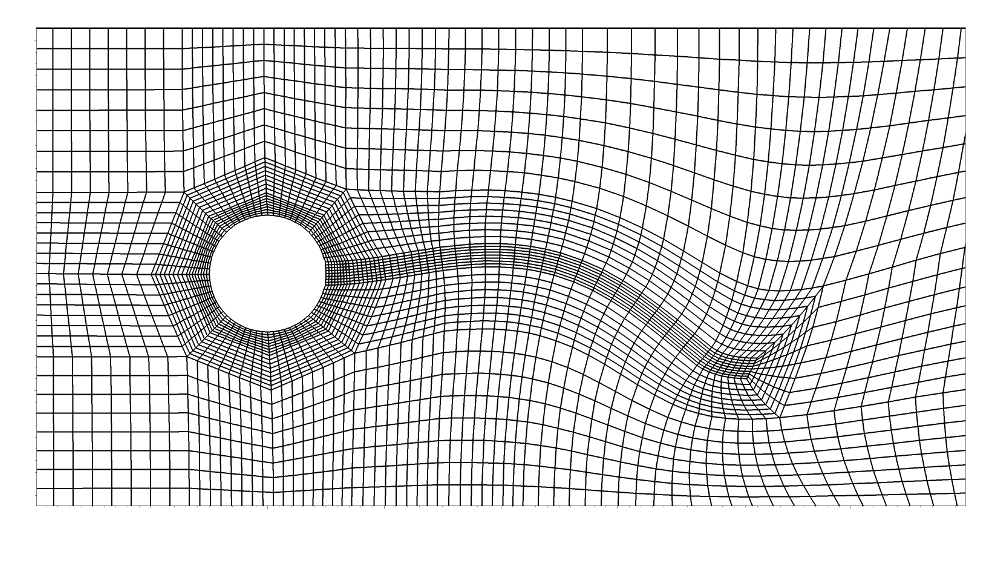
\includegraphics[width=6cm]{Pictures/visit_fsi_2_CNn_t_2e-2_global_3_biharmonic_mesh8070_scale.png}}
{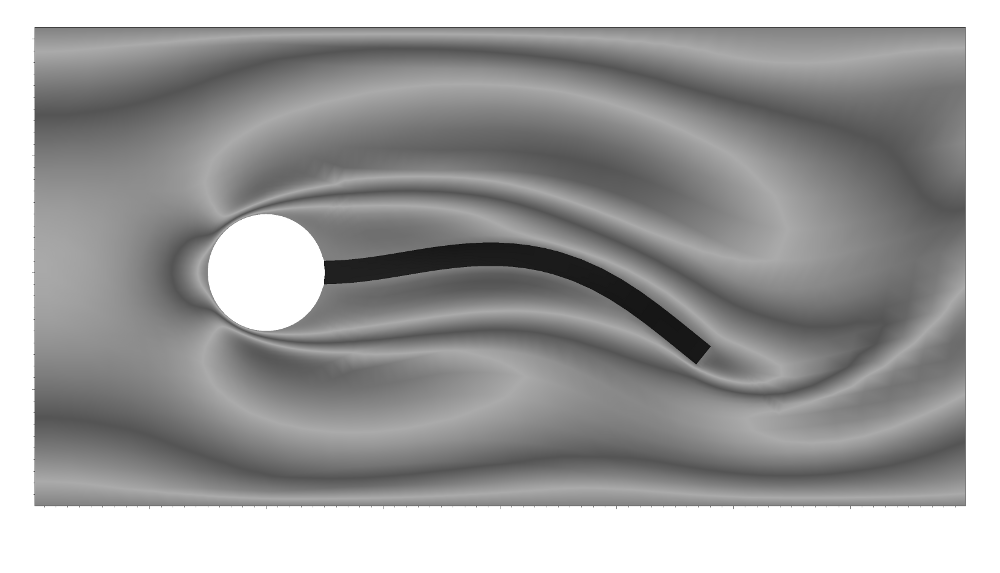
\includegraphics[width=6cm]{Pictures/visit_fsi_2_CNn_t_2e-2_global_3_biharmonic_x_velo8070_scale.png}}
\caption{FSI 2 test case: mesh (left) and velocity profile in vertical 
direction (right) at time $t=16.14s$.}
\label{res:fsi_2_mesh_and_x_velo}
\end{figure}

\begin{figure}
\centering
{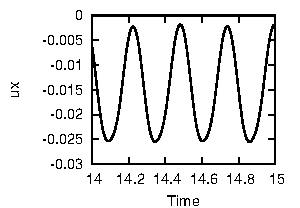
\includegraphics[width=5.8cm]{Pictures/ux_FSI_2_FS_t_3e-2_t_15e-3_global_2_Hron_grid.pdf}}
{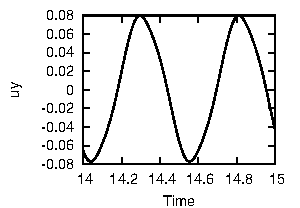
\includegraphics[width=5.8cm]{Pictures/uy_FSI_2_FS_t_3e-2_t_15e-3_global_2_Hron_grid.pdf}}
{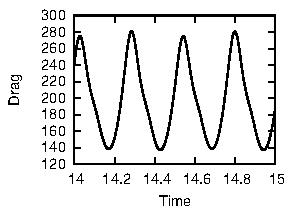
\includegraphics[width=5.8cm]{Pictures/Drag_fluid_FSI_2_FS_t_3e-2_t_15e-3_global_2_Hron_grid.pdf}}
{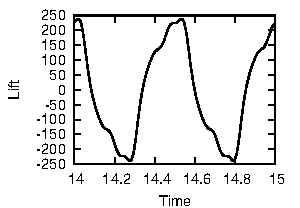
\includegraphics[width=5.8cm]{Pictures/Lift_fluid_FSI_2_FS_t_3e-2_t_15e-3_global_2_Hron_grid.pdf}}
\caption{FSI 2: the deflections of the beam, $u_x(A)$ and $u_y(A)$ (in $cm$), and 
the drag and the lift evaluation (in $kg/m\,s^2$) are displayed versus
time (in $s$).
} 
\label{res:results_ux_and_uy_fsi_2}
\end{figure}


\subsection{Compliance minimization}
Results already obtained.

\subsection{Goal-oriented mesh refinement for Navier-Stokes}
Has to be computed.

\subsection{Dirichlet Velocity, Neumann Pressure, and
Periodic Boundary Conditions}
I do not know.

%%%%%%%%%%%%%%%%%%%%%%%%%%%%%%%%%%%%%%%%%%%
\section{Conclusions and Outlook}
\label{conclusions}
In this article, we described the features 
and applications of the DOpElib project, which 
was initiated at the Heidelberg University in 2010.
Specifically, the applications cover a broad 
spectrum of numerical exmamples motivated 
by different disciplines. 
Currently, we are developing concepts for the efficient 
numerical solution of time-dependent optimization
problems governed by PDEs. 
\todo{Was wollen wir noch in den nächsten 1-2 Jahren erreichen?}



%%%%%%%%%%%%%%%%%%%%%%%%%%%%%%%%%%%%%%%%%%%
\section*{Acknowledgment}
The second author thanks Rolf Rannacher from
the Institute for Applied mathematics at the 
Heidelberg University for financial suppport. 




%%%%%%%%%%%%%%%%%%%%%%%%%%%%%%%%%%%%%%%%%%%
%\bibliographystyle{abbrvnat}
\bibliographystyle{acmsmall}
\bibliography{lit}
%


\end{document}


